\bta{$ 2019 $ 年普通高等学校招生全国统一考试(全国 \lmd{1} 卷)}

\begin{center}
\heiti 
\zihao{4}
物理部分
\end{center}
\vspace{1em}


\begin{enumerate}
\heiti
\renewcommand{\labelenumi}{\arabic{enumi}.}
% A(\Alph) a(\alph) I(\Roman) i(\roman) 1(\arabic)
%设定全局标号series=example	%引用全局变量resume=example
%[topsep=-0.3em,parsep=-0.3em,itemsep=-0.3em,partopsep=-0.3em]
%可使用leftmargin调整列表环境左边的空白长度 [leftmargin=0em]
\item[一、]
选择题:本题共 $ 8 $ 小题,每小题 $ 6 $ 分。在每小题给出的四个选项中,第 $ 1 \sim 5 $ 题只有一项符合
题目要求,第 $ 6 \sim 8 $ 题有多项符合题目要求。全部选对的得 $ 6 $ 分,选对但不全的得 $ 3 $ 分,有选
错的得 $ 0 $ 分。




\end{enumerate}


\begin{enumerate}
\renewcommand{\labelenumi}{\arabic{enumi}.}
% A(\Alph) a(\alph) I(\Roman) i(\roman) 1(\arabic)
%设定全局标号series=example	%引用全局变量resume=example
%[topsep=-0.3em,parsep=-0.3em,itemsep=-0.3em,partopsep=-0.3em]
%可使用leftmargin调整列表环境左边的空白长度 [leftmargin=0em]
\item
氢原子能级示意图如图所示。光子能量在 $ 1.63 \ eV \sim 3.10 \ eV $ 的光为可见光。要使处于基态 $ (n=1) $
的氢原子被激发后可辐射出可见光光子,最少应给氢原子提供的能量为 \xzanswer{A} 



\begin{figure}[h!]
\centering
\includesvg[width=0.23\linewidth]{picture/svg/908}
\end{figure}



\fourchoices
{$ 12.09 \ eV $}
{$ 10.20 \ eV $}
{$ 1.89 \ eV $}
{$ 1.5leV $}



\item
如图,空间存在一方向水平向右的匀强电场,两个带电小球 $ P $ 和 $ Q $ 用相同的绝缘细绳悬挂在水
平天花板下,两细绳都恰好与天花板垂直,则 \xzanswer{D} 

\begin{figure}[h!]
\centering
\includesvg[width=0.2\linewidth]{picture/svg/909}
\end{figure}

\fourchoices
{$ P $ 和 $ Q $ 都带正电荷}
{$ P $ 和 $ Q $ 都带负电荷}
{$ P $ 带正电荷,$ Q $ 带负电荷}
{$ P $ 带负电荷,$ Q $ 带正电荷}


\newpage
\item
最近,我国为“长征九号”研制的大推力新型火箭发动机联试成功,这标志着我国重型运载火箭
的研发取得突破性进展。若某次实验中该发动机向后喷射的气体速度约为 $ 3 \ km/s $,产生的推力
约为 $ 4.8 \times 10^{6} \ N $,则它在 $ 1 \ s $ 时间内喷射的气体质量约为 \xzanswer{B} 


\fourchoices
{$1.6 \times 10^{2} \ \mathrm{kg}$}
{$1.6 \times 10^{3} \ \mathrm{kg}$}
{$1.6 \times 10^{5}\ \mathrm{kg}$}
{$1.6 \times 10^{6}\ \mathrm{kg}$}

\banswer{

}


\item 
如图,等边三角形线框 $ LMN $ 由三根相同的导体棒连接而成,固定于匀强磁场中,线框平面与
磁感应强度方向垂直,线框顶点 $ M $ 、 $ N $ 与直流电源两端相接,已如导体棒 $ MN $ 受到的安培力
大小为 $ F $ ,则线框 $ LMN $ 受到的安培力的大小为 \xzanswer{B} 

\begin{figure}[h!]
\centering
\includesvg[width=0.23\linewidth]{picture/svg/910}
\end{figure}

\fourchoices
{$ 2F $}
{$ 1.5F $}
{$ 0.5F $}
{$ 0 $}

\banswer{

}


\item
如图,篮球架下的运动员原地垂直起跳扣篮,离地后重心上升的最大高度为 $ H $ 。上升第一个$\frac{H}{4}$
所用的时间为 $ t_{1} $ ,第四个$\frac{H}{4}$所用的时间为 $ t_{2} $ 。不计空气阻力,则 $\frac{t_{2}}{t_{1}}$ 满足 \xzanswer{C} 

\begin{figure}[h!]
\centering
\includesvg[width=0.23\linewidth]{picture/svg/911}
\end{figure}

\fourchoices
{$1<\frac{t_{2}}{t_{1}}<2$}
{$2<\frac{t_{2}}{t_{1}}<3$}
{$ 3<\frac{t_{2}}{t_{1}}<4$}
{$4<\frac{t_{2}}{t_{1}}<5$}

\banswer{

}

\newpage
\item
如图,一粗糙斜面固定在地面上,斜面顶端装有一光滑定滑轮。一细绳跨过滑轮,其一端悬挂
物块 $ N $。另一端与斜面上的物块 $ M $ 相连,系统处于静止状态。现用水平向左的拉力缓慢拉动 $ N $,
直至悬挂 $ N $ 的细绳与竖直方向成 $ 45 ^{ \circ } $。已知 $ M $ 始终保持静止,则在此过程中 \xzanswer{BD} 

\begin{figure}[h!]
\centering
\includesvg[width=0.33\linewidth]{picture/svg/912}
\end{figure}

\fourchoices
{水平拉力的大小可能保持不变}
{$ M $ 所受细绳的拉力大小一定一直增加}
{$ M $ 所受斜面的摩擦力大小一定一直增加}
{$ M $ 所受斜面的摩擦力大小可能先减小后增加}

\banswer{

}


\item
空间存在一方向与纸面垂直、大小随时间变化的匀强磁场,其边界如图($ a $)中虚线 $ MN $ 所示,
一硬质细导线的电阻率为 $ r $ 、横截面积为 $ S $ ,将该导线做成半径为 $ r $ 的圆环固定在纸面内,圆
心 $ O $ 在 $ MN $ 上。 $ t=0 $ 时磁感应强度的方向如图($ a $)所示,磁感应强度 $ B $ 随时间 $ t $ 的变化关系
如图($ b $)所示,则在 $ t=0 $ 到 $ t= t_{1} $ 的时间间隔内 \xzanswer{BC} 

\begin{figure}[h!]
\centering
\includesvg[width=0.5\linewidth]{picture/svg/913}
\end{figure}


\fourchoices
{圆环所受安培力的方向始终不变}
{圆环中的感应电流始终沿顺时针方向}
{圆环中的感应电流大小为$\frac{B_{0} r S}{4 t_{0} \rho}$}
{圆环中的感应电动势大小为$\frac{B_{0} \pi r^{2}}{4 t_{0}}$}

\banswer{

}

\newpage
\item
在星球 $ M $ 上将一轻弹簧竖直固定在水平桌面上,把物体 $ P $ 轻放在弹簧上端, $ P $ 由静止向下运
动,物体的加速度 $ a $ 与弹簧的压缩量 $ x $ 间的关系如图中实线所示。在另一星球 $ N $ 上用完全相
同的弹簧,改用物体 $ Q $ 完成同样的过程,其 $ a-x $ 关系如图中虚线所示,假设两星球均为质量
均匀分布的球体。已知星球 $ M $ 的半径是星球 $ N $ 的 $ 3 $ 倍,则 \xzanswer{AC} 

\begin{figure}[h!]
\centering
\includesvg[width=0.33\linewidth]{picture/svg/914}
\end{figure}

\fourchoices
{$ M $ 与 $ N $ 的密度相等}
{$ Q $ 的质量是 $ P $ 的 $ 3 $ 倍}
{$ Q $ 下落过程中的最大动能是 $ P $ 的 $ 4 $ 倍}
{$ Q $ 下落过程中弹簧的最大压缩量是 $ P $ 的 $ 4 $ 倍}


\begin{enumerate}[leftmargin=-2em]
\renewcommand{\labelenumii}{}
% A(\Alph) a(\alph) I(\Roman) i(\roman) 1(\arabic)
%可使用leftmargin调整列表环境左边的空白长度
\item
\btd{二、非选择题}
\end{enumerate}

\begin{enumerate}[leftmargin=-2em]
\renewcommand{\labelenumii}{}
% A(\Alph) a(\alph) I(\Roman) i(\roman) 1(\arabic)
%可使用leftmargin调整列表环境左边的空白长度
\item
\btd{(一)必考题}
\end{enumerate}

\item
($ 5 $ 分)某小组利用打点计时器对物块沿倾斜的长木板加速下滑时的运动进行研究。物块拖动纸
带下滑,打出的纸带一部分如图所示。已知打点计时器所用交流电的频率为 $ 50 \ Hz $,纸带上标
出的每两个相邻点之间还有 $ 4 $ 个打出的点未画出。在 $ A $、$ B $、$ C $、$ D $、$ E $ 五个点中,打点计时器
最先打出的是
\tk{A} 
点,在打出 $ C $ 点时物块的速度大小为
\tk{$ 0.233 $} 
$ m/s $(保留 $ 3 $ 位有效数字);物
块下滑的加速度大小为
\tk{$ 0.75 $} 
$ m/s^{2} $ (保留 $ 2 $ 位有效数字)。
\begin{figure}[h!]
\centering
\includesvg[width=0.83\linewidth]{picture/svg/915}
\end{figure}



\newpage
\item 
($ 10 $ 分)某同学要将一量程为 $ 250 \ \mu A $ 的微安表改装为量程为 $ 20 \ mA $ 的电流表。该同学测得微
安表内阻为 $ 1200 \ \Omega $,经计算后将一阻值为 $ R $ 的电阻与该微安表连接,进行改装。然后利用一
标准毫安表,根据图($ a $)所示电路对改装后的电表进行检测(虚线框内是改装后的电表)。
% TODO: \usepackage{graphicx} required
\begin{figure}[h!]
\centering
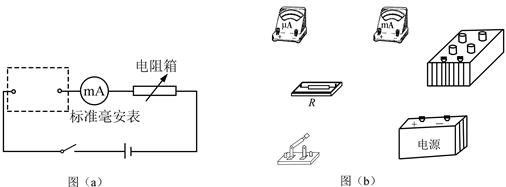
\includegraphics[width=0.83\linewidth]{picture/screenshot019}
\end{figure}


\begin{enumerate}
\renewcommand{\labelenumi}{\arabic{enumi}.}
% A(\Alph) a(\alph) I(\Roman) i(\roman) 1(\arabic)
%设定全局标号series=example	%引用全局变量resume=example
%[topsep=-0.3em,parsep=-0.3em,itemsep=-0.3em,partopsep=-0.3em]
%可使用leftmargin调整列表环境左边的空白长度 [leftmargin=0em]
\item
根据图($ a $)和题给条件,将($ b $)中的实物连接。


%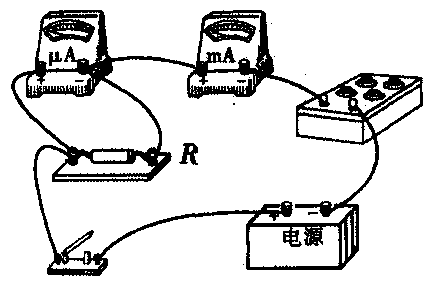
\includegraphics[width=0.7\linewidth]{picture/screenshot020}



\item 
当标准毫安表的示数为 $ 16.0 \ mA $ 时,微安表的指针位置如图($ c $)所示,由此可以推测出所
改装的电表量程不是预期值,而是 \underlinegap 。(填正确答案标号)
\begin{figure}[h!]
\centering
\includesvg[width=0.46\linewidth]{picture/svg/916}
\end{figure}

\fourchoices
{$ 18 \ mA $}
{$ 21 \ mA $}
{$ 25 \ mA $}
{$ 28 \ mA $}




\item 
产生上述问题的原因可能是 \underlinegap 。(填正确答案标号)

\fourchoices
{微安表内阻测量错误,实际内阻大于 $ 1200 \ \Omega $}
{微安表内阻测量错误,实际内阻小于 $ 1200 \ \Omega $}
{$ R $ 值计算错误,接入的电阻偏小}
{$ R $ 值计算错误,接入的电阻偏大}



\item 
要达到预期目的,无论测得的内阻值是否正确,都不必重新测量,只需要将阻值为 $ R $ 的电
阻换为一个阻值为 $ kR $ 的电阻即可,其中 $ k= $ \underlinegap 。

\end{enumerate}


\tk{
\begin{enumerate}
%\renewcommand{\labelenumi}{\arabic{enumi}.}
% A(\Alph) a(\alph) I(\Roman) i(\roman) 1(\arabic)
%设定全局标号series=example	%引用全局变量resume=example
%[topsep=-0.3em,parsep=-0.3em,itemsep=-0.3em,partopsep=-0.3em]
%可使用leftmargin调整列表环境左边的空白长度 [leftmargin=0em]
\item
C
\item 
AC
\item 
$\frac{99}{79}$
\end{enumerate}
} 


\newpage
\item 
($ 12 $ 分)如图,在直角三角形 $ OPN $ 区域内存在匀强磁场,磁感应强度大小为 $ B $ 、方向垂直于
纸面向外。一带正电的粒子从静止开始经电压 $ U $ 加速后,沿平行于 $ x $ 辅的方向射入磁场;一
段时间后,该粒子在 $ OP $ 边上某点以垂直于 $ x $ 轴的方向射出。已知 $ O $ 点为坐标原点,$ N $ 点在 $ y $
轴上,$ OP $ 与 $ x $ 轴的夹角为 $ 30 ^{ \circ } $,粒子进入磁场的入射点与离开磁场的出射点之间的距离为 $ d $ ,
不计重力。求:



\begin{enumerate}
\renewcommand{\labelenumi}{\arabic{enumi}.}
% A(\Alph) a(\alph) I(\Roman) i(\roman) 1(\arabic)
%设定全局标号series=example	%引用全局变量resume=example
%[topsep=-0.3em,parsep=-0.3em,itemsep=-0.3em,partopsep=-0.3em]
%可使用leftmargin调整列表环境左边的空白长度 [leftmargin=0em]
\item
带电粒子的比荷;



\item 
带电粒子从射入磁场到运动至 $ x $ 轴的时间。




\end{enumerate}
\begin{figure}[h!]
\flushright
\includesvg[width=0.28\linewidth]{picture/svg/917}
\end{figure}

\banswer{
\begin{enumerate}
\renewcommand{\labelenumi}{\arabic{enumi}.}
% A(\Alph) a(\alph) I(\Roman) i(\roman) 1(\arabic)
%设定全局标号series=example	%引用全局变量resume=example
%[topsep=-0.3em,parsep=-0.3em,itemsep=-0.3em,partopsep=-0.3em]
%可使用leftmargin调整列表环境左边的空白长度 [leftmargin=0em]
\item
$\frac{q}{m}=\frac{4 U}{B^{2} d^{2}}$
\item 
$t=\frac{B d^{2}}{4 U}\left(\frac{\pi}{2}+\frac{\sqrt{3}}{3}\right)$

\end{enumerate}


}


\newpage
\item 
($ 20 $ 分)竖直面内一倾斜轨道与一足够长的水平轨道通过一小段光滑圆弧平滑连接,小物块 $ B $
静止于水平轨道的最左端,如图($ a $)所示。 $ t=0 $ 时刻,小物块 $ A $ 在倾斜轨道上从静止开始下
滑,一段时间后与 $ B $ 发生弹性碰撞(碰撞时间极短);当 $ A $ 返回到倾斜轨道上的 $ P $ 点(图中未
标出)时,速度减为 $ 0 $,此时对其施加一外力,使其在倾斜轨道上保持静止。物块 $ A $ 运动的 $ v-t $
图像如图($ b $)所示,图中的 $ v_{1} $ 和 $ t_{1} $ 均为未知量。已知 $ A $ 的质量为 $ m $ ,初始时 $ A $ 与 $ B $ 的高度差
为 $ H $ ,重力加速度大小为 $ g $,不计空气阻力。



\begin{enumerate}
\renewcommand{\labelenumi}{\arabic{enumi}.}
% A(\Alph) a(\alph) I(\Roman) i(\roman) 1(\arabic)
%设定全局标号series=example	%引用全局变量resume=example
%[topsep=-0.3em,parsep=-0.3em,itemsep=-0.3em,partopsep=-0.3em]
%可使用leftmargin调整列表环境左边的空白长度 [leftmargin=0em]
\item
求物块 $ B $ 的质量;



\item 
在图($ b $)所描述的整个运动过程中,求物块 $ A $ 克服摩擦力所做的功;


\item 
已知两物块与轨道间的动摩擦因数均相等,在物块 $ B $ 停止运动后,改变物块与轨道间的动
摩擦因数,然后将 $ A $ 从 $ P $ 点释放,一段时间后 $ A $ 刚好能与 $ B $ 再次碰上。求改变前面动摩擦
因数的比值。





\end{enumerate}
\begin{figure}[h!]
\flushright
\includesvg[width=0.65\linewidth]{picture/svg/918}
\end{figure}

\banswer{
\begin{enumerate}
\renewcommand{\labelenumi}{\arabic{enumi}.}
% A(\Alph) a(\alph) I(\Roman) i(\roman) 1(\arabic)
%设定全局标号series=example	%引用全局变量resume=example
%[topsep=-0.3em,parsep=-0.3em,itemsep=-0.3em,partopsep=-0.3em]
%可使用leftmargin调整列表环境左边的空白长度 [leftmargin=0em]
\item
$m^{\prime}=3 m$
\item 
$W=\frac{2}{15} m g H$
\item 
$\frac{\mu}{\mu^{\prime}}=\frac{11}{9}$
\end{enumerate}


}



\newpage
\begin{enumerate}[leftmargin=-2em]
\renewcommand{\labelenumii}{}
% A(\Alph) a(\alph) I(\Roman) i(\roman) 1(\arabic)
%可使用leftmargin调整列表环境左边的空白长度
\item
\btd{(二)选考题}
\end{enumerate}


\item 

[物理—选修 $ 3 $–$ 3 $]($ 15 $ 分)


\begin{enumerate}
\renewcommand{\labelenumi}{\arabic{enumi}.}
% A(\Alph) a(\alph) I(\Roman) i(\roman) 1(\arabic)
%设定全局标号series=example	%引用全局变量resume=example
%[topsep=-0.3em,parsep=-0.3em,itemsep=-0.3em,partopsep=-0.3em]
%可使用leftmargin调整列表环境左边的空白长度 [leftmargin=0em]
\item
($ 5 $ 分)某容器中的空气被光滑活塞封住,容器和活塞绝热性能良好,空气可视为理想气体。
初始时容器中空气的温度与外界相同,压强大于外界。现使活塞缓慢移动,直至容器中的空
气压强与外界相同。此时,容器中空气的温度 \tk{低于} (填“高于”“低于”或“等于”)外界
温度,容器中空气的密度 \tk{大于} (填“大于”“小于”或“等于”)外界空气的密度。



\item 
($ 10 $ 分)热等静压设备广泛应用于材料加工中。该设备工作时,先在室温下把惰性气体用
压缩机压入到一个预抽真空的炉腔中,然后炉腔升温,利用高温高气压环境对放入炉腔中的
材料加工处理,改善其性能。一台热等静压设备的炉腔中某次放入固体材料后剩余的容积为
$ 0.13 \ m^{3} $ ,炉腔抽真空后,在室温下用压缩机将 $ 10 $ 瓶氩气压入到炉腔中。已知每瓶氩气的容
积为 $ 3.2 \times 10^{-2} \ m^{3} $ ,使用前瓶中气体压强为 $ 1.5 \times 10^{7} \ Pa $,使用后瓶中剩余气体压强为
$ 2.0 \times 10^{6} \ Pa $;室温温度为 $ 27 \ \celsius $。氩气可视为理想气体。
\begin{enumerate}
\renewcommand{\labelenumiii}{\roman{enumiii}.}
% A(\Alph) a(\alph) I(\Roman) i(\roman) 1(\arabic)
%设定全局标号series=example	%引用全局变量resume=example
%[topsep=-0.3em,parsep=-0.3em,itemsep=-0.3em,partopsep=-0.3em]
%可使用leftmargin调整列表环境左边的空白长度 [leftmargin=0em]
\item
求压入氩气后炉腔中气体在室温下的压强;
\item 
将压入氩气后的炉腔加热到 $ 1227 \ \celsius $,求此时炉腔中气体的压强。




\end{enumerate}
\banswer{
\begin{enumerate}
\renewcommand{\labelenumi}{\arabic{enumi}.}
% A(\Alph) a(\alph) I(\Roman) i(\roman) 1(\arabic)
%设定全局标号series=example	%引用全局变量resume=example
%[topsep=-0.3em,parsep=-0.3em,itemsep=-0.3em,partopsep=-0.3em]
%可使用leftmargin调整列表环境左边的空白长度 [leftmargin=0em]
\item
$p_{2}=3.2 \times 10^{7} \ \mathrm{Pa}$
\item 
$p_{3}=1.6 \times 10^{8} \mathrm{Pa}$

\end{enumerate}


}






\end{enumerate}



\newpage
\item 

[物理一选修 $ 3-4 $]($ 15 $ 分)


\begin{enumerate}
\renewcommand{\labelenumi}{\arabic{enumi}.}
% A(\Alph) a(\alph) I(\Roman) i(\roman) 1(\arabic)
%设定全局标号series=example	%引用全局变量resume=example
%[topsep=-0.3em,parsep=-0.3em,itemsep=-0.3em,partopsep=-0.3em]
%可使用leftmargin调整列表环境左边的空白长度 [leftmargin=0em]
\item
($ 5 $ 分)一简谐横波沿 $ x $ 轴正方向传播,在 $t=\frac{T}{2}$
时刻,该波的波形图如图($ a $)所示, $ P $ 、
$ Q $ 是介质中的两个质点。图($ b $)表示介质中某质点的振动图像。下列说法正确的是 \tk{CDE} 
(填
正确答案标号。选对 $ 1 $ 个得 $ 2 $ 分,选对 $ 2 $ 个得 $ 4 $ 分,选对 $ 3 $ 个得 $ 5 $ 分。每选错 $ 1 $ 个扣 $ 3 $ 分,
最低得分为 $ 0 $ 分)
\begin{figure}[h!]
\centering
\includesvg[width=0.53\linewidth]{picture/svg/919}
\end{figure}



\fivechoices
{质点 $ Q $ 的振动图像与图($ b $)相同}
{在 $ t=0 $ 时刻,质点 $ P $ 的速率比质点 $ Q $ 的大}
{在 $ t=0 $ 时刻,质点 $ P $ 的加速度的大小比质点 $ Q $ 的大}
{平衡位置在坐标原点的质点的振动图像如图($ b $)所示}
{在 $ t=0 $ 时刻,质点 $ P $ 与其平衡位置的距离比质点 $ Q $ 的大}


\item 
($ 10 $ 分)如图,一艘帆船静止在湖面上,帆船的竖直桅杆顶端高出水面 $ 3 \ m $。距水面 $ 4 \ m $
的湖底 $ P $ 点发出的激光束,从水面出射后恰好照射到桅杆顶端,该出射光束与竖直方向的夹
角为 $ 53 ^{ \circ } $(取 $ \sin 53 ^{ \circ } =0.8 $)。已知水的折射率为$ \frac{ 4 }{ 3 } $。



\begin{enumerate}
\renewcommand{\labelenumiii}{\roman{enumiii}.}
% A(\Alph) a(\alph) I(\Roman) i(\roman) 1(\arabic)
%设定全局标号series=example	%引用全局变量resume=example
%[topsep=-0.3em,parsep=-0.3em,itemsep=-0.3em,partopsep=-0.3em]
%可使用leftmargin调整列表环境左边的空白长度 [leftmargin=0em]
\item
求桅杆到 $ P $ 点的水平距离;
\item 
船向左行驶一段距离后停止,调整由 $ P $ 点发出的激光束方向,当其与竖直方向夹角为 $ 45 ^{ \circ } $
时,从水面射出后仍然照射在桅杆顶端,求船行驶的距离。




\end{enumerate}
\begin{figure}[h!]
\flushright
\includesvg[width=0.55\linewidth]{picture/svg/920}
\end{figure}


\banswer{
\begin{enumerate}
\renewcommand{\labelenumi}{\arabic{enumi}.}
% A(\Alph) a(\alph) I(\Roman) i(\roman) 1(\arabic)
%设定全局标号series=example	%引用全局变量resume=example
%[topsep=-0.3em,parsep=-0.3em,itemsep=-0.3em,partopsep=-0.3em]
%可使用leftmargin调整列表环境左边的空白长度 [leftmargin=0em]
\item
$x=7 \ \mathrm{m}$

\item 
$=x^{\prime}=(6 \sqrt{2}-3) \ m \approx 5.5 \ m$
\end{enumerate}


}



\end{enumerate}




\end{enumerate}


